% TODO list:
% - Add sage and magma to refs.
% - Include thanks? anyone else?
% - How will code be included, snippets or on disk??
% - Think about typography

% Structure:
% - Introduction
% - Background
% - Problem
% -  History??
% -- Statements
% -- Quadratics
% -- Cubics?
% -- Cocyclics
% -- Monogenics
% -- General absolute
% -- General relatives
% - Applications to elliptics over Q
% - Conclusion

% Include project managementy bits
% Practical considerations, lines of code, sage vs magma python etc.

\documentclass[a4paper,abstracton,bibtotoc]{scrreprt}

\author{Alex J. Best \\ Supervised by Dr. Lassina Demb\'el\'e}
\date{2014}
\title{Finding orders with prescribed index in number fields}

\usepackage{amsmath, amssymb, amsfonts, amsthm, hyperref, listings, tikz, algorithm2e, graphicx}
\usepackage[utf8]{inputenc}
\usepackage[T1]{fontenc}
\usepackage[english]{babel}

\theoremstyle{definition}
\newtheorem{thm}{Theorem}
\newtheorem{lem}{Lemma}
\newtheorem{cor}{Corollary}
\newtheorem{prop}{Proposition}
\newtheorem{defn}{Definition}
\newtheorem{defns}{Definitions}
\newtheorem{prob}{Problem}
\newtheorem{ex}{Example}
\newtheorem{rem}{Remark}
\newtheorem{nota}{Notation}
\newtheorem{alg}{Algorithm}

\setcounter{tocdepth}{3}

\lstset{
basicstyle=\footnotesize,       % the size of the fonts that are used for the code
showspaces=false,               % show spaces adding particular underscores
showstringspaces=false,         % underline spaces within strings
showtabs=false,                 % show tabs within strings adding particular underscores
frame=single,           % adds a frame around the code
captionpos=b,           % sets the caption-position to bottom
breaklines=true,        % sets automatic line breaking
breakatwhitespace=false,    % sets if automatic breaks should only happen at whitespace
}

\graphicspath{{img/}}

\newcommand{\QQ}{\mathbf{Q}}
\newcommand{\RR}{\mathbf{R}}
\newcommand{\CC}{\mathbf{C}}
\newcommand{\ZZ}{\mathbf{Z}}
\renewcommand{\O}{\mathcal{O}}

\DeclareMathOperator{\Orders}{Orders}
\DeclareMathOperator{\Ann}{Ann}

\begin{document}
\maketitle

\begin{abstract}
%TODO insert very small backstory, orders are objects in ant here ..
Orders in number fields are common objects of study in algebraic number theory.
Here we develop methods to obtain all orders with a specified index inside another given one.
The performance, both theoretically and in implementations of these methods is discussed.
We also apply these techniques to problems relating to elliptic curves over the rational numbers.

\smallskip
\noindent \textbf{Keywords.} Number theory, algebraic number theory, elliptic curves, number fields, algorithms.
\end{abstract}

\tableofcontents

\chapter{Introduction}
This report deals with the algorithmic solution of a problem arising from algebraic number theory. 
Other interesting situations to which this algorithm can be applied are also looked at.

We first go through the background material needed to motivate, define and describe the solution of our problems in chapter~\ref{chap:background}.
Then in section~\ref{sec:statements} we move on to the problems themselves and discuss the interest in studying them.
After this in the rest of chapter~\ref{chap:prob} we detail the techniques used to solve the problems considered, starting with some special cases before moving onto more general results.
Finally in section~\ref{sec:ell} we move on to some interesting applications of these methods to the study of elliptic curves.

\chapter{Background material}
\label{chap:background}

In this section we fix several definitions and important results from algebraic number theory and commutative algebra.
We assume only fairly basic knowledge of abstract algebra, such as the notions of groups, rings and fields.

The results given here are well known and are used throughout the rest of the report.

\section{Commutative algebra}
We introduce several notions and results that will be useful to us throughout the report, proofs for those results not proved here can be found in many textbooks on commutative algebra, such as \cite{am} or \cite{matsumura}.

All rings here are commutative with an identity element.
\begin{defn}[Module]
Given a ring $R$ we define an \emph{$R$-module} $M$ to be an abelian group under addition, with a scalar multiplication map $\cdot \colon R\times M \to M$ satisfying
\begin{align*}
1\cdot m &= m \; &&\forall m\in M \\
r_1\cdot(r_2 \cdot m) &= (r_1r_2)\cdot m \; &&\forall r_1,r_2\in R,\; m\in M \\
r\cdot(m_1 + m_2) &= r\cdot m_1 + r\cdot m_2 \; &&\forall r\in R, \; m_1,m_2\in M \\
(r_1 + r_2)\cdot m &= r_1\cdot m + r_2\cdot m \; &&\forall r_1,r_2\in R, \; m_1\in M
\end{align*}
\end{defn}

We often refer to elements of the ring $R$ as \emph{scalars}.

From now on we will omit the notation $\cdot$ for scalar multiplication as it will be clear from context when the multiplication is taking place in the ring $R$ or on a module $M$.
We will also not make explicit the ring $R$ involved if it is not relevant to the discussion at hand, instead referring simply to a \emph{module}.

The most common modules we will use here will be $\ZZ$-modules such as:
\begin{ex}

\end{ex}
In fact every abelian group can be given a $\ZZ$-module structure so of course they are ubiquitous in all commutative algebra, nevertheless it is useful to think of the modules used here in terms of $\ZZ$ rather than as abstract abelian groups.
We now list some standard definitions that are used to talk about how different modules relate to one another and describe ways of constructing new modules from old.

\begin{defn}[Module homomorphism]
Given $R$-modules $M_1$ and $M_2$ a map $f\colon M_1 \to M_2$ satisfying
\begin{align*}
f(rm) &= rf(m) &&\text{ for all $r\in R$, $m\in M_1$}\\
f(m + m') &= f(m) + f(m')&&\text{ for all $m,m'\in M_1$}
\end{align*}
is called an \emph{$R$-module homomorphism} or simply a \emph{module homomorphism} when the ring is clear.
\end{defn}

\begin{defn}[Isomorphism of modules]
Two $R$-modules $M_1$ and $M_2$ are said to be \emph{isomorphic} is there exists a bijective module homomorphism between them. 
In this case we write $M_1\cong M_2$.
\end{defn}

Module isomorphism is an equivalence relation on the class of all modules and so we often think of two isomorphic modules as being the same, just written in a different manner.

\begin{defn}[Submodule]
A \emph{submodule} $N$ of a module $M$ is a module whose elements all belong to $M$ and whose operations are the same as those from $M$ on the elements on $N$.
\end{defn}

\begin{defn}[Quotient module]
The \emph{quotient module} of two $R$-modules $M$ and $N$ with $M$ a submodule of $N$ is defined to be the quotient abelian group under addition $N/
M$ with scalar multiplication given by
\[
r\cdot(m + N) = rm + N\text{ for all $r\in R$, $m\in M$}.
\]
\end{defn}

\begin{defn}[Index]
Given a module $M$ that is a submodule of a module $N$ the \emph{index} of $M$ in $N$, denoted $[N:M]$ is the size of the quotient module $N / M$.
\end{defn}

\begin{defn}[Direct sum]
Given two $R$-modules $M_1$ and $M_2$ we define their \emph{direct sum} (denoted $\oplus$) to be the module with element set $M_1 \times M_2$ and operations given by the operations of $M_1$ and $M_2$ performed elementwise. i.e.
\begin{align*}
r\cdot(m_1,m_2) &= (r\cdot m_1, r\cdot m_2)\\
(m_1,m_2) + (m_1',m_2') &= (m_1 + m_1',m_2+m_2').
\end{align*}
\end{defn}

Not that this is in general distinct from when we have $M_1$ and $M_2$ submodules of some module $N$ and write
\[
M_1 + M_2 = \{m_1 + m_2 \mid m_1\in M_1,\ m_2\in M_2\}.
\]
For example with this elementwise addition we have $M + M = M$ for any module $M$, whereas $M\oplus M$ is not isomorphic to $M$ unless $M$ is the trivial module containing only a zero element and no others.

The well known isomorphism theorems also hold for modules, we require only two.

\begin{thm}[First isomorphism theorem for modules]
Given a surjective module homomorphism $f\colon M \to N$ the kernel of $f$ is a submodule of $M$ and
\[
M/\ker(f) \cong N.
\]
\end{thm}

\begin{thm}[Third isomorphism theorem for modules]
Given a chain of submodules $M_1 \subseteq M_2 \subseteq M_3$ the quotient module $M_2/M_1$ is a submodule of $M_3/M_1$ and we have an isomorphism
\[
(M_3/M_1)/(M_2/M_1) \cong (M_3/M_2).
\]
\end{thm}

An easy consequence of this relating the indices of submodules is worth noting.

\begin{cor}
\label{cor:indexmult}
Given a chain of submodules $M_1 \subseteq M_2 \subseteq M_3$ we have
\[
[M_3:M_1] = [M_3:M_2][M_2:M_1].
\]
\end{cor}

\minisec{}
We now define a property of modules that makes them easier to work with and importantly easier to do computations with.

\begin{defn}[Finitely generated]
An $R$-module $M$ is \emph{finitely} generated if there is a \emph{finite} set $B\subset M$ such that any $m\in M$ can be written as
\[m = \sum_{b\in B} \alpha_b b\]
for some coefficients $\alpha_b \in R$.
\end{defn}

\begin{defn}[Torsion submodule]
The \emph{torsion submodule} $M_\text{tors}$ of an $R$-module $M$ is the set
\[
\{m\in M \mid \exists\; r \in R\setminus 0 \text{ such that } rm = 0\}.
\]
This is the set of elements that are killed by some non-zero scalar.
As implied by the name this is always submodule of $M$.
\end{defn}

A module $M$ is called a torsion module if $M_\text{tors} = M$, and torsion-free if $M_\text{tors} = 0$.

% TODO generalise to module over PID
% TODO direct sum/prod

\begin{defn}[Rank of a $\ZZ$-module]
Given a $\ZZ$-module $M$ we can always write $M = M_\text{tors} \oplus \ZZ^r$ for some unique $r\in \ZZ_{\ge 0}$.
This $r$ is called the \emph{rank} of the $\ZZ$-module.
\end{defn}

\begin{ex}
\[M = \ZZ^2 = \{(a,b)\mid a,b\in \ZZ\}\]
is a torsion free $\ZZ$ module. Let
\[N = \{(2c,0) \mid c\in\ZZ\} \cong \ZZ\]
be a submodule of $M$.
Then the quotient module
\[M/N \cong (\ZZ/2\ZZ)\times \ZZ\]
has torsion submodule equal to $\ZZ/2\ZZ$ and is of rank 1.
\end{ex}

\section{Algebraic number theory}

Algebraic number began with the study of algebraic numbers and their uses in solving Diophantine equations but has since expanded to encompass a huge amount of mathematics involving the use of algebraic techniques to tackle number theoretic problems. %TODO ????
As above, more details about anything not proved here can be found in any of the many texts on algebraic number theory, for example \cite{neukirch}, \cite{lang}.

\begin{defn}[Number field]
A \emph{number field} $K$ is a field that is also a finite dimensional $\QQ$-vector space.
\end{defn}

\begin{ex}\label{ex:quad}
We write $\QQ(\sqrt{3})$ for the smallest field containing both $\QQ$ and $\sqrt{3}$, it is clear that the set
\[
\{a + b\sqrt{3}\mid a,b \in \QQ\}
\]
must be contained in such a field.
But we can also see that this set is closed under addition, subtraction, multiplication and non-zero division, and hence this set is the field $\QQ(\sqrt{3})$.

Here we see that $\QQ(\sqrt{3})$ has dimension 2 as a vector space over $\QQ$.
\end{ex}

\begin{defn}[Degree of a number field]
The dimension of a number field $K$ as a $\QQ$ vector space is called the \emph{degree} of $K$, denoted $[K:\QQ]$.

We say that number fields of degree 2, such as in example~\ref{ex:quad} above are \emph{quadratic}.
Similarly degree 3 number fields are called \emph{cubic}.
\end{defn}

\minisec{}
The following few definitions are central to the whole problem.

A number field will often have a large number of subrings, which may be of interest to us, however not all subrings are as nice as we would like them to be.
So we distinguish some subrings that have desirable properties and single them out for study.

\begin{defn}[Order]
An \emph{order} of a number field $K$ is a subring of $K$ that is finitely generated as a $\ZZ$-module, and of rank equal to the degree of $K$ (this is the maximal rank).
\end{defn}

%TODO finite basis

\begin{defn}[Ring of integers]
The \emph{ring of integers}, denoted $\ZZ_K$, of a number field $K$ is the unique maximal order.
\end{defn}

The terminology for this ring comes from the fact that its behaviour is analogous to the way $\ZZ$ behaves inside $\QQ$.

We can use the notion of index in a variety of situations here, such as considering the index of a module in another, the index of a module in a ring, etc. %TODO ????

\begin{ex}
\[
[\ZZ\cdot 1 + \ZZ\cdot \sqrt{2} : \ZZ \cdot 1 + \ZZ \cdot 2\sqrt{2}] = 2.
\]
\end{ex}

\begin{ex}
As we will see later the maximal order of a quadratic number field is easy to determine.
For example in figure~\ref{fig:sageord} one embedding into the complex plane of the ring of integers of $\QQ[x]/(x^2 + 19)\cong \QQ(\sqrt{-19})$ is shown.
Highlighted in black is a suborder of index 3 in this order.
\begin{figure}
\centering
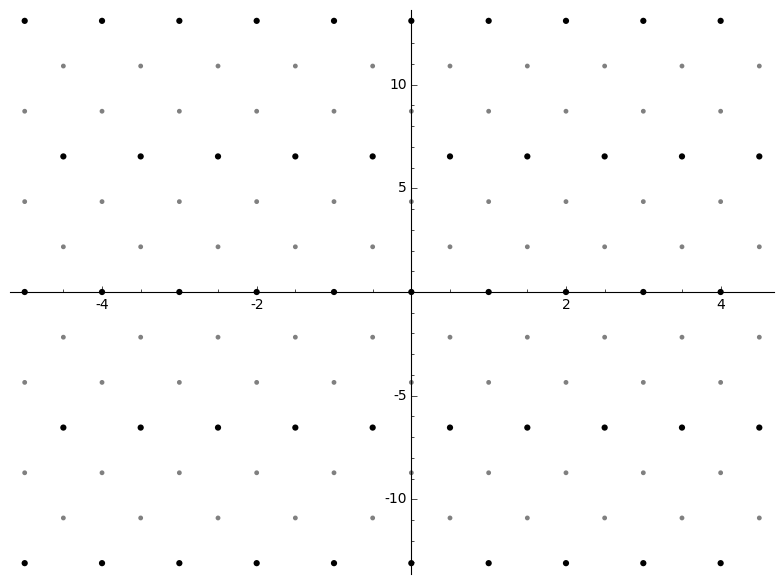
\includegraphics[scale=0.6]{sageord}
\caption{\label{fig:sageord} An embedding in $\CC$ of the ring of integers of $\QQ(\sqrt{-19})$.}
\end{figure}
\end{ex}

%P.<x> = QQ[]
%K = NumberField(x^2 + 19, 'a')
%ZK = K.maximal_order()
%OK = K.order(3*ZK.0)
%print ZK.basis()
%f = K.embeddings(CC)[0]
%pts = []
%pts2 = []
%for x in range(-10,10):
%    for y in range(-10,10):
%        if f(x*ZK.0 + y*ZK.1).imag().abs() < 15: 
%            pts.append(f(x*ZK.0 + y*ZK.1))
%        if f(x*OK.0 + y*OK.1).imag().abs() < 15: 
%            pts2.append(f(x*OK.0 + y*OK.1))
%
%list_plot(pts,color="gray",size=12) + list_plot(pts2,color="black",size=20)

\section{Elliptic curves}
We now introduce the background material relevant to elliptic curves, one of the intended applications of these methods.
This is not required for the main problem discussed in chapter~\ref{chap:prob}, but section~\ref{sec:ell} uses these ideas heavily.
As with the above sections everything here can be found in textbooks on elliptic curves (such as \cite{knapp}), we just move quickly to the parts relevant to us in this section.
%TODO more refs

Given an elliptic curve $E$ and a field $K$ we let $E(K)$ be the set of points in $K^2$ satisfying the equation defining $E$, along with an extra point $\infty$.
This extra point is called the point at infinity, the reasons for its inclusion in the set should become clear later.

\begin{ex}
Let 
\[
E \colon y^2 + 2xy + y = x^3 - 2x + 3.
\]
Then we can see for example that $(1,(\sqrt{17}-3)/2)\in E(\RR) \subset E(\CC)$ as the coordinates satisfy the equation defining the curve.

We can plot the real points of this curve, such a plot is shown in figure~\ref{fig:ec}.
This plot of the real points is typical for an elliptic curves though there can easily be two connected components rather than one as in this case.
\begin{figure}
\centering
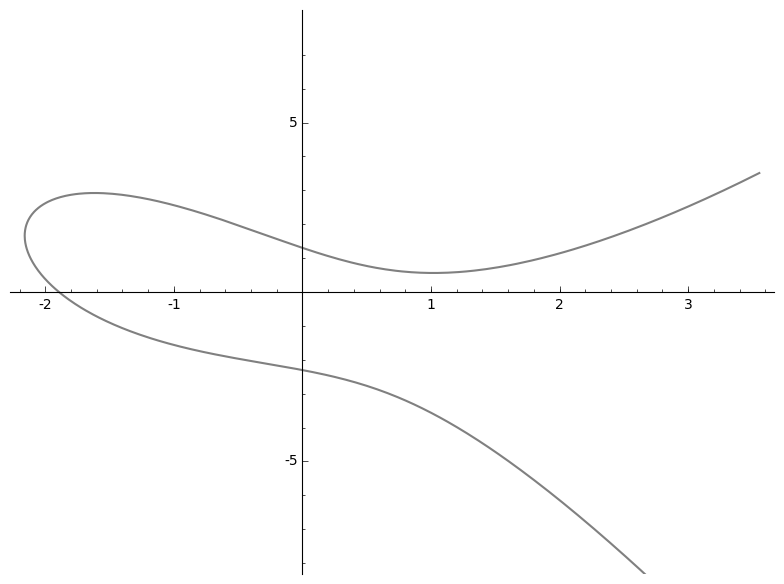
\includegraphics[scale=0.6]{sageec}
\caption{\label{fig:ec}$E(\RR)$.}
\end{figure}
\end{ex}

One of the things that makes elliptic curves so interesting to study is the fact that we can define a natural way of adding points of the curve over some field, with this definition the set of points on the curve becomes a group.

\begin{defn}[Group law]
\end{defn}

With this definition of addition the set of points of $E$ over some field $K$ is a group, and moreover this group is abelian.
From now on we will denote the point $\infty\in E(K)$ as $0$, but still refer to it as \emph{at infinity}.

As remarked above any abelian group can be regarded as a $\ZZ$-module $M$ in a natural way by letting 
\[n\cdot z = \underbrace{z + z + \cdots + z}_\text{$n$ times},\text{ for } n\in\ZZ_{\ge 0},\ z\in M\]
and letting $n\cdot z = (-n)\cdot(-z)$ for negative $n\in \ZZ$.
With this idea in mind $E(K)_\text{tors}$ is the set of points of $E$ defined over $K$ that can be added to themselves some finite number of times to get the point at infinity.
This is often called the \emph{torsion subgroup} of $E$.
It turns out that when $K = \QQ$ there are only a finite number of groups that $E(\QQ)_\text{tors}$ can be.

\begin{thm}[Mazur's torsion theorem]
\label{thm:tors}
Given an elliptic curve $E$ defined over the rationals $E(\QQ)_\text{tors}$ is one of:
\[
\ZZ/i\ZZ,\text{ for } i \in\{1,2,\ldots,9,10,12\}\text{ or }
\ZZ/2\ZZ \times \ZZ/2i\ZZ,\text{ for } i \in\{1,2,3,4\}.
\]
\end{thm}

In fact similar results have been obtained for quadratic fields too, for more detail on what is known about the torsion subgroup of an elliptic curve over a number field see \cite{sutherland}.

Sometimes it is necessary to talk about smaller subgroups of this group whose elements have order dividing some fixed $n$ and so we introduce the following definition.
\begin{defn}[$n$-division points]
For some $n\in\ZZ$ the set of \emph{$n$-division points} of $E$ over $K$ is
\[
E(K)[n] = \{P\in E(K) \mid nP = 0\}.
\]
\end{defn}
Although by theorem~\ref{thm:tors} $E(\QQ)_\text{tors}$ cannot be large it is still useful to consider the $n$-division points of a curve and we will use this group later.
%If $K = \QQ$ we can see from theorem~\ref{thm:tors} that $E(\QQ)[n]$ is likely to be interesting for $n\in\{2,3,4\}$.

\minisec{}
We are now ready to state in precise terms the project aimed to solve and to detail the methods used in its solution.

\chapter{The problem}
\label{chap:prob}
\section{Statement}
\label{sec:statements}

The aim of the project was to find a general method to solve the following problem, and moreover to find efficient algorithms that can solve the problem on any given inputs.

\begin{prob}
Given an order $R$ of an absolute number field $K$ and an integer $I$ find the set
\[\left\{ \O\subseteq R \mid \O\text{ is a suborder},\ [R:\O] = I\right\}.\]
\end{prob}

To find a suborder we really mean compute a $\ZZ$ basis for the order, as such a basis defines an order completely.
With $R$ and $I$ as in the proposition we introduce the following notation to refer to the set we are looking for.

\[\Orders(R,I) = \left\{ \O\subseteq R \mid \O\text{ is a suborder},\ [R:\O] = I\right\}.\]

\minisec{}
One very natural extension of the above problem is to consider relative extensions of number fields.
More precisely we wish to study the following problem.

\begin{prob} % TODO check this is really what I mean
Given an extension of number fields $L|K$, a $\ZZ_K$-order $R$ of $\ZZ_L$ and an integer $I$ find the set
\[\left\{ \O\subseteq R \mid \O\text{ is a $\ZZ_K$-suborder},\ [R:\O] = I\right\}.\]
\end{prob}

We now detail some methods to solve this problem in varying generality.

\section{Quadratic number fields}

Quadratic number fields are the simplest non-trivial number fields and they have a large amount of structure which can often make them easier to work with than more general number fields.
As we will see, in this case the solution of our problem is very simple.

It is well known \cite{lang} that the ring of integers of a quadratic field $K = \QQ(\sqrt{d})$ for $d$ non-square always takes the form
\[\ZZ_K = \ZZ + \ZZ\alpha,\text{ with } \alpha =\begin{cases}
\sqrt{d}&\text{ if $d\equiv 2,3\pmod{4}$},\\
\frac{1+\sqrt{d}}{2}&\text{ if $d\equiv 1\pmod{4}$}.
\end{cases}\]

Indeed there is so little room for manoeuvre here that the following result on the structure of an order holds in this case.

\begin{prop}
\label{prop:quadord}
Every order $\O$ of a quadratic number field can be expressed as
\[\O = \ZZ + \ZZ f\alpha\]
for some $f\in \ZZ$, $\alpha$ as above.
\end{prop}

For a proof see \cite[pp. 133--134]{cox}.

\begin{defn}
The $f$ appearing in the above proposition is called the \emph{conductor} of the order $\O$.
Later we shall abuse this definition slightly by redefining the conductor to generalise this concept.
\end{defn}

Now it is clear that
\[
[\ZZ + \ZZ\alpha : \ZZ + \ZZ f \alpha] = |\ZZ/f\ZZ| = |f|.
\]
So we have an incredibly simple solution for quadratic number fields, there is exactly one order of a given index in $\ZZ_K$.
Hence in the quadratic case can say the following.

\begin{prop}
If $\ZZ_K = \ZZ + \ZZ\alpha$ and $R = \ZZ + \ZZ m\alpha$ then
\[
\Orders(R, I) = \{\ZZ + \ZZ Im\alpha\}.
\]
\end{prop}
\begin{proof}
This follows immediately from the above description of orders of $K$ (proposition~\ref{prop:quadord}) and the fact that the index is multiplicative (corollary \ref{cor:indexmult}).
\end{proof}
%TODO make sure we get the solution to match the problem statement! arbitrary starting order!

%TODO cubic????

\section{Monogenic orders}

We now look at a special class of orders that have been studied extensively by other authors.

\begin{defn}[Monogenic order]
An order of the form $\ZZ[\alpha]$ for some algebraic integer $\alpha$ is called \emph{monogenic}.
\end{defn}

Monogenic orders are easier to work with and are common in algebraic number theory.
The ease of computing with them comes from the fact that
\[
\ZZ[\alpha] = \ZZ + \ZZ\alpha + \ZZ\alpha^2 + \cdots + \ZZ\alpha^{n-1}
\]
and so $\{1,\alpha,\ldots,\alpha^{n-1}\}$ is a basis for $\ZZ[\alpha]$ as a $\ZZ$ module (here $n$ is $[K : \QQ]$).

%TODO explain niceness of monogenic orders etc

%TODO give examples of non-monogenic orders, orders with n-1 ring gens for any n??

%TODO explain that in some ways idea was to generalise this to arbitrary orders

\section{Cocyclic orders}
\label{sec:cocyc}
We recall some definitions and results given by Johannes Brakenhoff in his thesis \cite{brakenhoff}.
These will be helpful when considering the class of cocyclic orders, defined as follows.

\begin{defn}[Cocyclic order]
An order $\O$ of a number field $K$ is called \emph{cocyclic} if
\[
\ZZ_K/\O \cong \ZZ/m\ZZ,
\]
i.e. the quotient of the maximal order of the $K$ by $\O$ is a cyclic group.
\end{defn}

\begin{ex}
\label{ex:cocyc}
Let $K = \QQ[x]/(x^4 ) = \QQ(\alpha)$ be a number field and take %TODO fill in
\[
\O = \ZZ + \ZZ3\alpha + \ZZ9\alpha^2 + \ZZ3\alpha^3.
\]
Then as $\ZZ_K = \ZZ[\alpha]$ we have
\[
\ZZ_K/\O \cong 
\]
and so $\O$ is cocyclic.
\end{ex}

The following theorem which is a specialisation of \cite[Thm. 4.1]{brakenhoff} will allow us to find cocyclic orders very easily.
We include the proof here as it is quite instructive. %TODO generalise to all starting orders???

\begin{thm}
\label{thm:coresp}
Let $K$ be a number field and fix some $m\in\ZZ$ then let
\[
W = \{\O \text{ an order of } K\mid \ZZ_K/\O \cong \ZZ/m\ZZ\}
\]
and
\[
V = \{ J \text{ an ideal of }\ZZ_K \mid \ZZ_K/J \cong (\ZZ/m\ZZ)^2 \}.
\]
Then there is a bijection between $V$ and $W$ given by
\begin{align*}
f\colon W &\to V\\
\O &\mapsto \{a\in\ZZ_K \mid a\ZZ_K \subseteq \O \}
\end{align*}
and
\begin{align*}
g\colon V&\to W\\
J&\mapsto \ZZ + J.
\end{align*}
\end{thm}

\begin{proof}\cite[Thm. 4.1, pp. 35]{brakenhoff} %TODO 
We first show the maps are well defined.
$f(\O) = \Ann_{\ZZ_K}(\ZZ_K/\O)$ which is an ideal of $\ZZ_K$.
%As $\ZZ_K$ and $\O$ are rings we have that $f(\O)\ZZ_K \subset f(\O)$ and $f(\O) + f(\O) \subset f(O)$, hence $f(\O)$ is an ideal of $\ZZ_K$ and so in $W$.

\end{proof}

The image of $f$ above is still well defined for non-cocyclic orders and this ideal is known as the \emph{conductor} of $\O$.%TODO just defined for maximal?

The set $W$ above is the set of cocyclic orders of index $m$ and so we can find them by finding the corresponding ideals of $V$ and then simply adding in $\ZZ$.

\begin{alg}
\label{alg:cocyc}~\\
\begin{algorithm}[H] %TODO fix this, do we need to check if order?
Factor the ideals $p_i\O$ into prime ideals for the primes $p_i$ dividing $I^2$.\\
Using all possible factorisations of $I^2$ in $\ZZ$ and the norms of the prime ideals found above find all ideals in $\O$ of index $I^2$.\\
\For{all ideals $I$ found above}{
Let $M = \ZZ + I$.\\
\If{$M$ is of index}
{
add $M$ to the output.
}
}
\end{algorithm}
\end{alg}

However this is not a full solution of our problem as not all orders of number fields are cocyclic.

\begin{ex}
\label{ex:noncocyc}
With $K = $ (as in example~\ref{ex:cocyc}) and $\O = \ZZ + 9\ZZ_K$ we have
\[
\ZZ_K/\O = 
\]
and so $\O$ is not cocyclic.
\end{ex}

\section{General orders in absolute number fields}

We originally hoped that the correspondence between suborders and their conductors that exists in the quadratic case (theorem \ref{thm:coresp}) could be generalised to higher degree number fields.
However the direct generalisations of this result fail to hold even in degree 3 number fields.
We now give examples of some results that would be good for our purposes if true and explicit counter examples for each of them.
% TODO list some generalisations here


\subsection{The Hermite normal form}
The Hermite normal form of a matrix is ..

So in order 

\subsection{The basic algorithm}
%TODO how to check subring
\begin{alg}~\\
\begin{algorithm}[H]
\For{all HNF matrices $H$ of determinant $I$}{
Find the submodule $M$ of $\O$ corresponding to $H$.\\
\If{$M$ is a subring}
{
add $M$ to the output.
}
}
\end{algorithm}
\end{alg}
%TODO speed up including 1

\subsection{Making use of less general methods} %TODO cut this section :( / reduce as speedup is small
Given the results discussed in \ref{sec:cocyc} we can improve the performance of the above algorithm as follows.
\begin{alg}~\\
\begin{algorithm}[H]
Find cocyclic orders of index $I$ in $\O$ using algorithm~\ref{alg:cocyc}.\\
\For{all HNF matrices $H$ of determinant $I$}{
\If{$H$ is the matrix of a cocyclic order already found}
{
Move to the next matrix.
}
Find the submodule $M$ of $\O$ corresponding to $H$.\\
\If{$M$ is a subring}
{
add $M$ to the output.
}
}
\end{algorithm}
\end{alg}

\section{Relative number fields}


\section{Practical considerations}
Though the methods described above are the best we have been able to obtain so far from a theoretical perspective, when it comes down to computing examples in the real world there are a number of ideas and techniques we can use to reduce the time taken.

\subsection{Parallelisation}
Several stages of the algorithm for general orders can be naturally parallelised reducing the total time taken linearly with the number of threads used.
For example once the set of potential conductors has been computed the orders to which they correspond can all be computed in parallel.
Similarly the set of HNF matrices used can be computed in parallel and whether the modules they generate form rings or not can be checked simultaneously too.

\subsection{Timings}

\chapter{Applications}

Through the main problem itself is an interesting one which is worth studying in its own right we were also motivated to look at it by the potential applications to other questions within the same areas of mathematics.
% TODO are there more apps?
One of the most prominent areas in which a solution to the problem can be used is to answer questions about elliptic curves.
How a solution to the problem considered above can be applied in this case is detailed below, along with results obtained from the application of our methods there.

\section{Elliptic curves}
\label{sec:ell}
Given an elliptic curve defined over the rationals in long Weierstrass form, for example
\[E_l \colon y^2 + a_1xy + a_3y = x^3 + a_2x^2 + a_4x + a_6\text{ with }a_i \in \QQ,\]
we can find an isomorphic curve $E \colon y^2 = x^3 + a_2'x^2 + a_4'x + a_6'$, such a curve is said to be in \emph{short Weierstrass form}.

Given such a curve we can define a number field to help us study the torsion points of $E$.
\begin{defn}[$p$-division field]
For a prime $p$ the $p$-division field of $E$, denoted $\QQ(E[p])$ is obtained by taking all points $(x,y) \in E(\QQ)[p]\setminus 0\subset \QQ^2$ and adjoining the collection of each of their coordinates $x$ and $y$ to $\QQ$.
\end{defn}
As the torsion subgroup $E(\QQ)_\text{tors}$ is always finite there are at most finitely many elements that need adjoining to $\QQ$, so this field is fairly nice.

\minisec{}
Assuming that the curve $E$ has no rational 2-torsion points we must have no rational solution to $f = x^3 + ??$ and hence the polynomial is irreducible over $\QQ$.
We can then see that we have
\[
\QQ(E[2]) \cong \QQ[x]/(f).
\]
Letting $\alpha$ be the image of $x$ in the above quotient, we can see that $ \ZZ[\alpha]$ is an order of $\QQ(\alpha)\cong \QQ(E[2])$.


\chapter{Conclusion}
%TODO conclude, several variants developed all with advantages disadvantages

\section{Further work}
It seems likely that other properties of the orders we are looking for could be used to speed up the algorithms given above and so further investigations into both special cases and the general cases could yield results.
Further applications of these methods are certainly possible and it would be interesting to see what other areas these methods can be used in.

\section{Acknowledgements}
First and foremost I would like to thank Lassina Demb\'el\'e for his excellent guidance while I undertook the project.
I am also grateful to John Cremona for allowing me access to one of the Warwick number theory group's servers to run computations on.

%\chapter{Appendix: Code}

%Much of what was done has been implemented in both the Sage and Magma and so we provide annotated source code listings for the algorithms in both languages below.
 
%\section{Sage}
%\lstinputlisting[language=Python]{../sage/order_of_index.py}

%\section{Magma}
%\lstinputlisting[language=Pascal]{../magma/orderofindex.m}

\nocite{*}
\bibliographystyle{alpha}
\bibliography{biblio}

\end{document}
